\ifdefined\included
\else
\setcounter{chapter}{4} %% Numéro du chapitre précédent ;)
\dominitoc
\faketableofcontents
\fi

\chapter{Interactive Simulator}
\chaptermark{Interactive Simulator}
\label{chap:5}
\minitoc

\chapabstract{This chapter contains a technical description of an interactive simulator allowing human operators to collaborate with a simulated robot executing the policies described in the previous chapter. This simulator is used in the next chapter to conduct a user study to validate our approach.}

\section{Introduction}

In order to validate the approach presented in the previous chapter (\ref{chap:4}), we would like to be able to perform a task collaboratively with a simulated robot executing the produced policy. This allowed us to conduct a user study described in the next chapter (chap.~\ref{chap:6}) which validates our planning approach.


\begin{figure}
    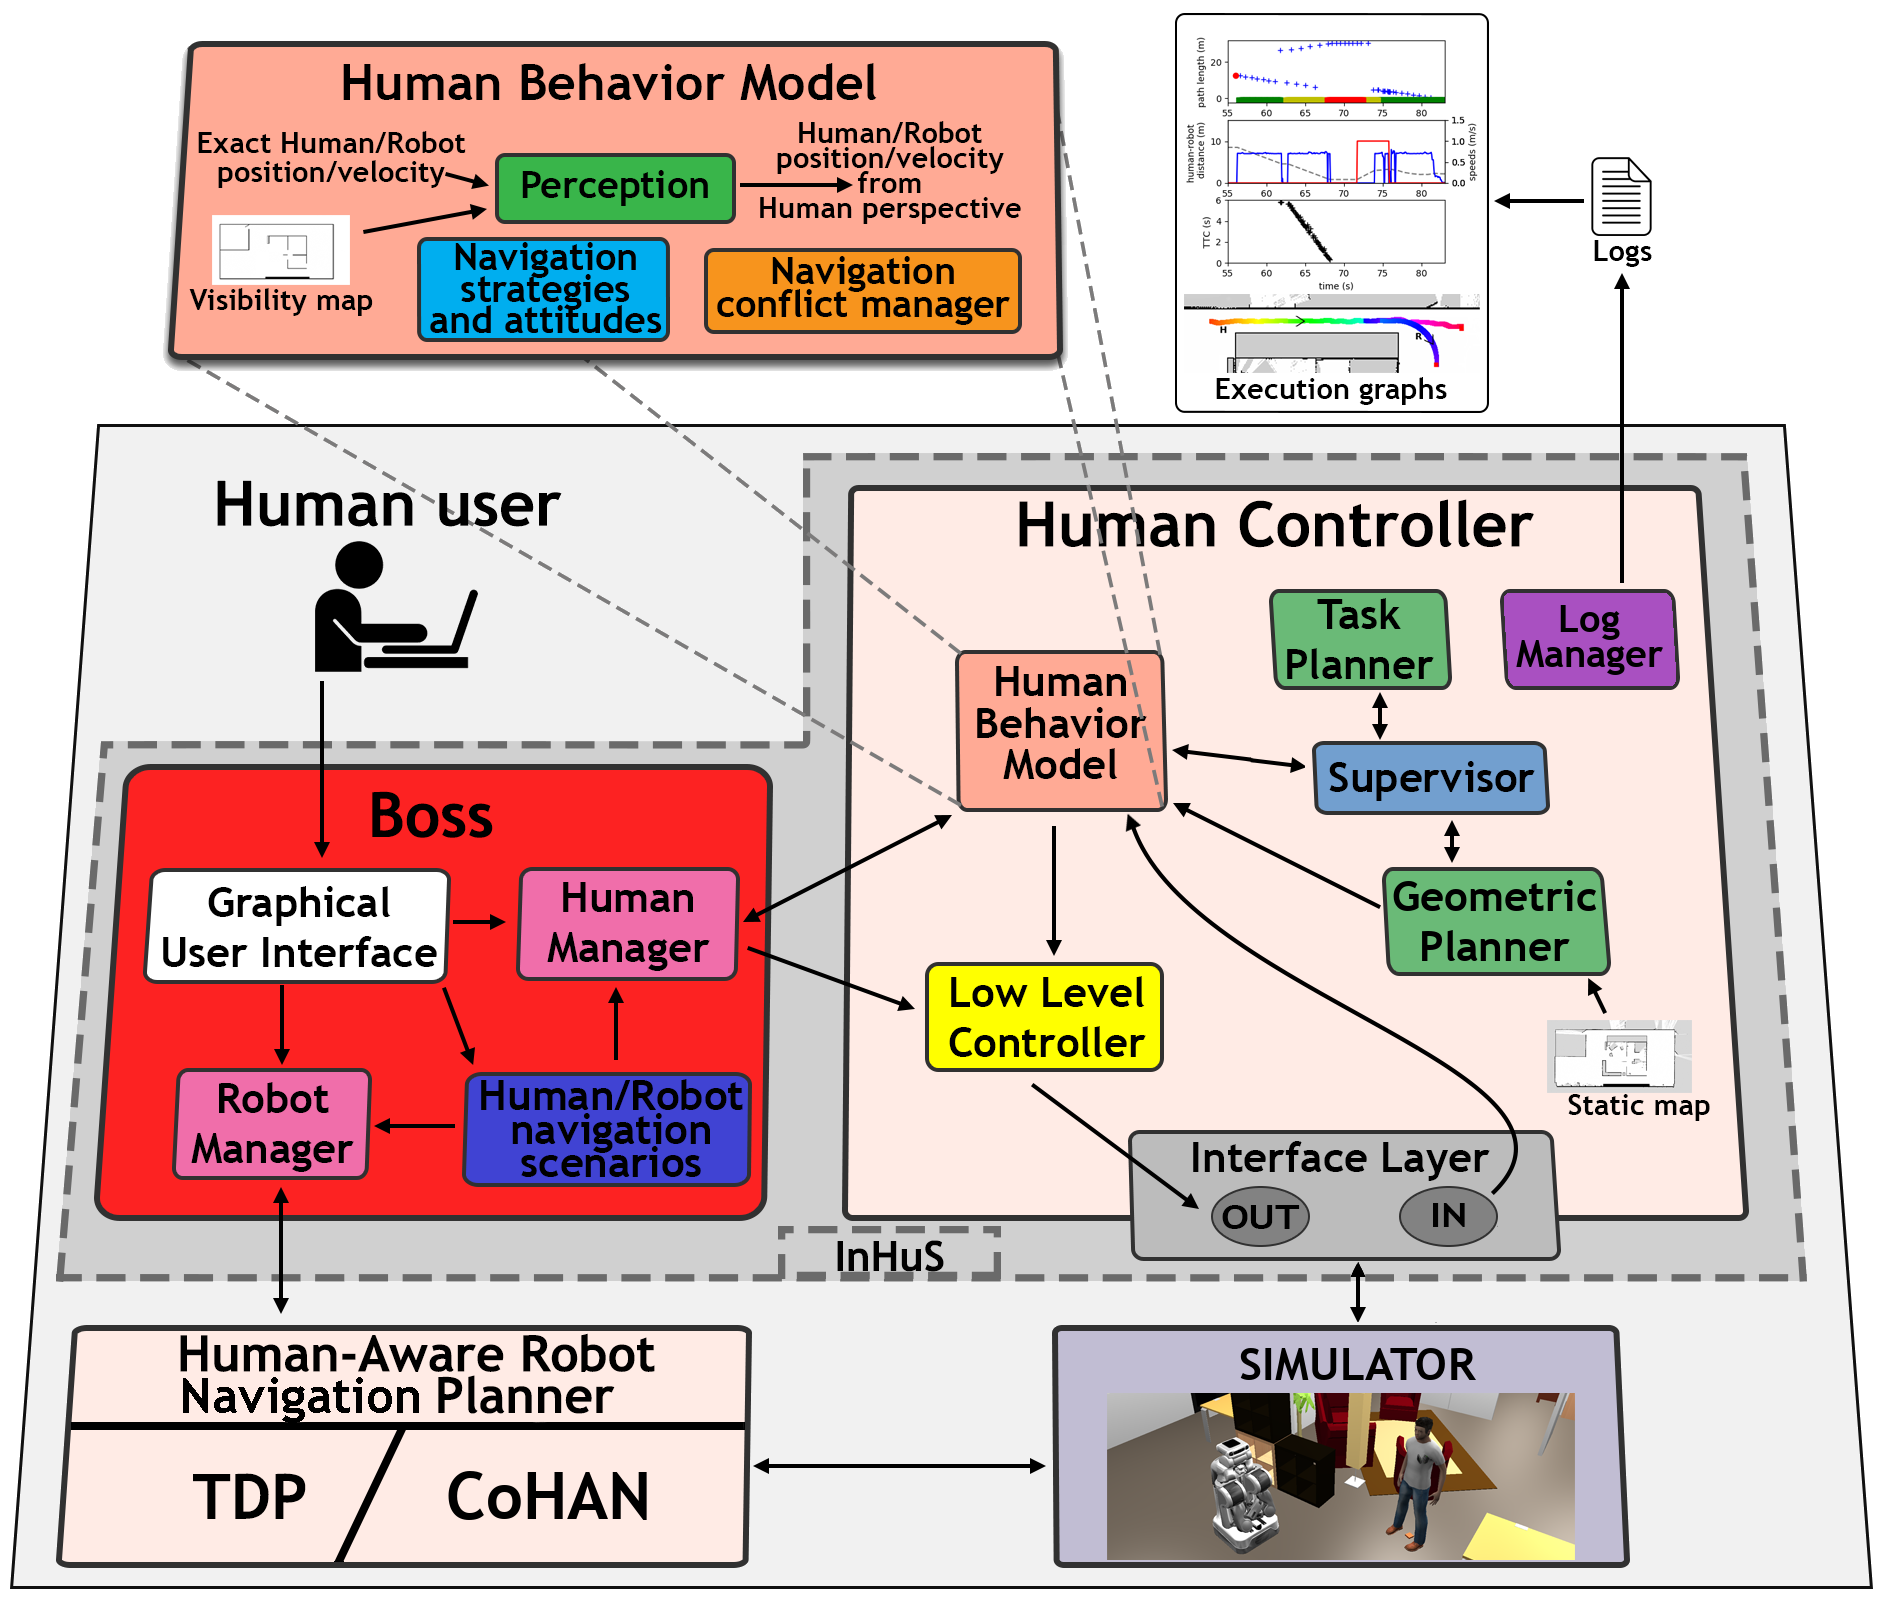
\includegraphics[width=\textwidth]{Chapter5/architecture.pdf}
    \caption{Overview of the Interactive Simulator's Architecture}
    \label{fig:architecture}
\end{figure}

This chapter is a technical description of the interactive simulator I developed. As depicted in fig.~\ref{fig:architecture}, it consists of several components detailed throughout this chapter. We describe the simulated scene corresponding to a BlocksWorld task similar to the one presented in the last chapter but with more cubes. After, the execution controller used is presented, corresponding to a refined and implemented version of the abstracted joint action execution model introduced in the last chapter. We continue by describing the different motion and simulation controllers used to interact with the simulator. Then, the Human-Machine Interface is presented, allowing participants to perform actions in the simulator. Finally, we present how the data retrieved during each execution are used to compute several metrics to evaluate the execution.  

\section{Simulated Scene}

This interactive simulator is based on the Gazebo Simulator. It is an open-source 3D simulator able to simulate articulated robots in a dynamic and complex environment.
This section describes all aspects directly linked to this existing 3D simulator our framework has been developed upon.

The static scene consists of a large room, with a ground and 4 walls, and a table placed in the center with two marks on its right side. The marks represent the locations where the cubes must be stacked. The agents are represented as follows. First, the human is represented only with a floating hand as the camera simulates a first-person point-of-view. Then we used a Tiago robot from PAL Robotics because it has an arm to manipulate its environment, a head to send gaze information and signals and because many related resources are available for it (3D models, controllers, tutorials). The human and the robot are facing each other, each from one opposite side of the table. Finally, colored cubes were disposed of on the table in three distinct zones. Cubes are either close to the edge of one of the agents, or they are in the middle of the table. This disposition influences the reachability of the agents as one agent can only reach cubes from their side (just in front of them) or the middle, but never from the other agent's side. This scene corresponds to one specific collaborative task, but another setup could be easily implemented. 

The Gazebo simulator can be integrated with the Robot Operating System (ROS) which is a set of software libraries and tools that help to build robot applications. The main pros of ROS are its ability to run several sub-programs in parallel and make them communicate with each other. Hence, the other components of the interactive simulator have been developed with ROS.

The overall scene is depicted in the figure~\ref{fig:simu_view}. The stacking goal is displayed in the top left corner and a text prompt is shown in the top right corner for the robot to communicate with the human.

\begin{figure}[h]
    \centering
    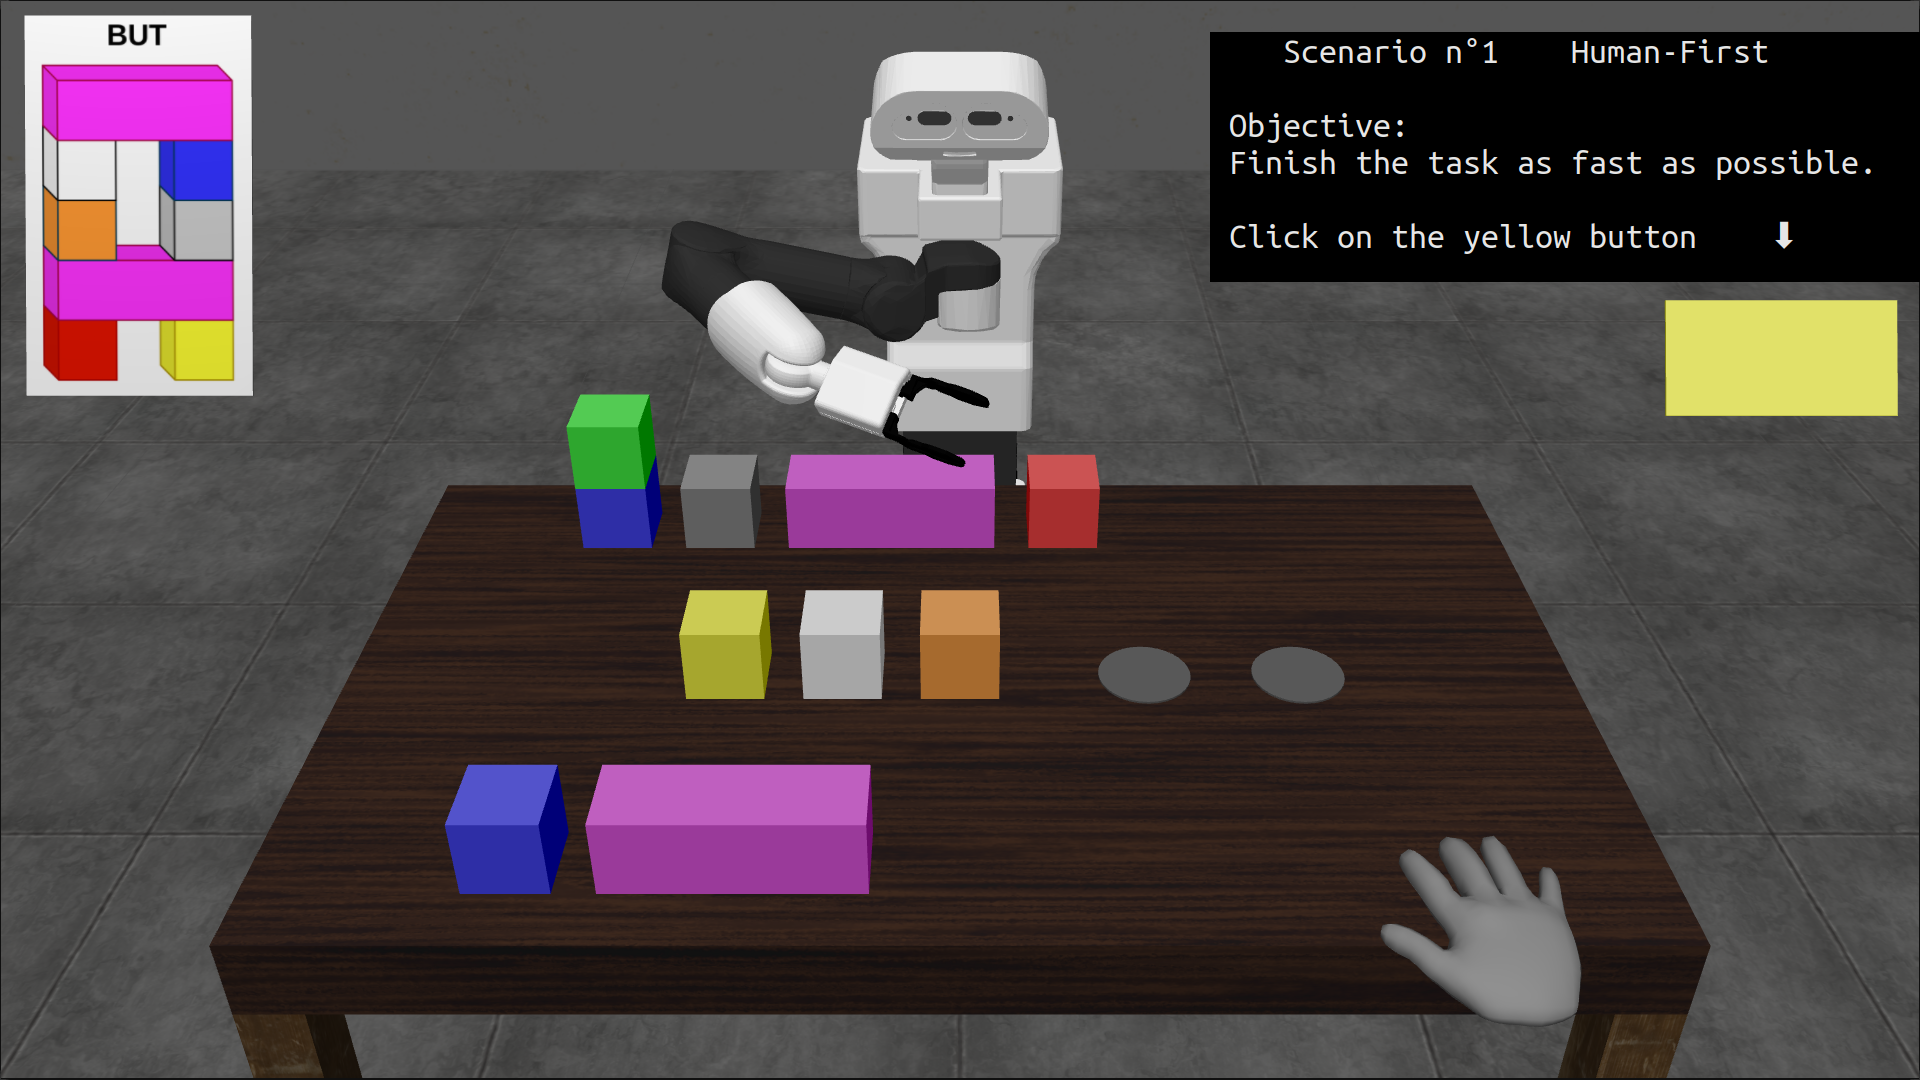
\includegraphics[width=\textwidth]{Chapter5/simu_screenshot.png}
    \caption{Participant view of the interactive simulator. Text prompt. Goal pattern. robot. table. cubes. stacking area. human hand.}
    \label{fig:simu_view}
\end{figure}


\section{Execution Controller - Joint Action Model for Execution}

The model of execution presented in the last chapter was simplified and used to explore further relevant courses of action. This allows for anticipating the possible coordination and complying with online human decisions. 
However, we need an execution controller that will supervise the execution of the produced policy. The execution model presented in the last chapter was simplified and abstracted to guide the planning algorithms. Here, we propose a refined and implemented model, matching the abstraction previously made, to be able to execute the produced robot policy and supervise its execution by synchronizing with the human.

The complete model is depicted in fig~\ref{fig:complete_model_exec}. On top of refining the `robot automaton' present in the abstracted version, it also models the human agent's behavior with another automaton that captures the possible decisions the human may make during execution. Additionally, this complete model makes all the social signals exchanged between the agents explicit and shows how they are used for coordination. These differences are discussed in detail below. This execution controller takes as input the solution DAG produced by the chap.~\ref{chap:4} approach. Then, the controller progresses from the initial state to a goal in the solution graph. The controller handles the state transitions, step by step, by sending and synchronizing on social cues. Thanks to this and the associated simulator, we now have a durative task execution with an effectice effect on a simulated environment.


\begin{figure}
    \centering
    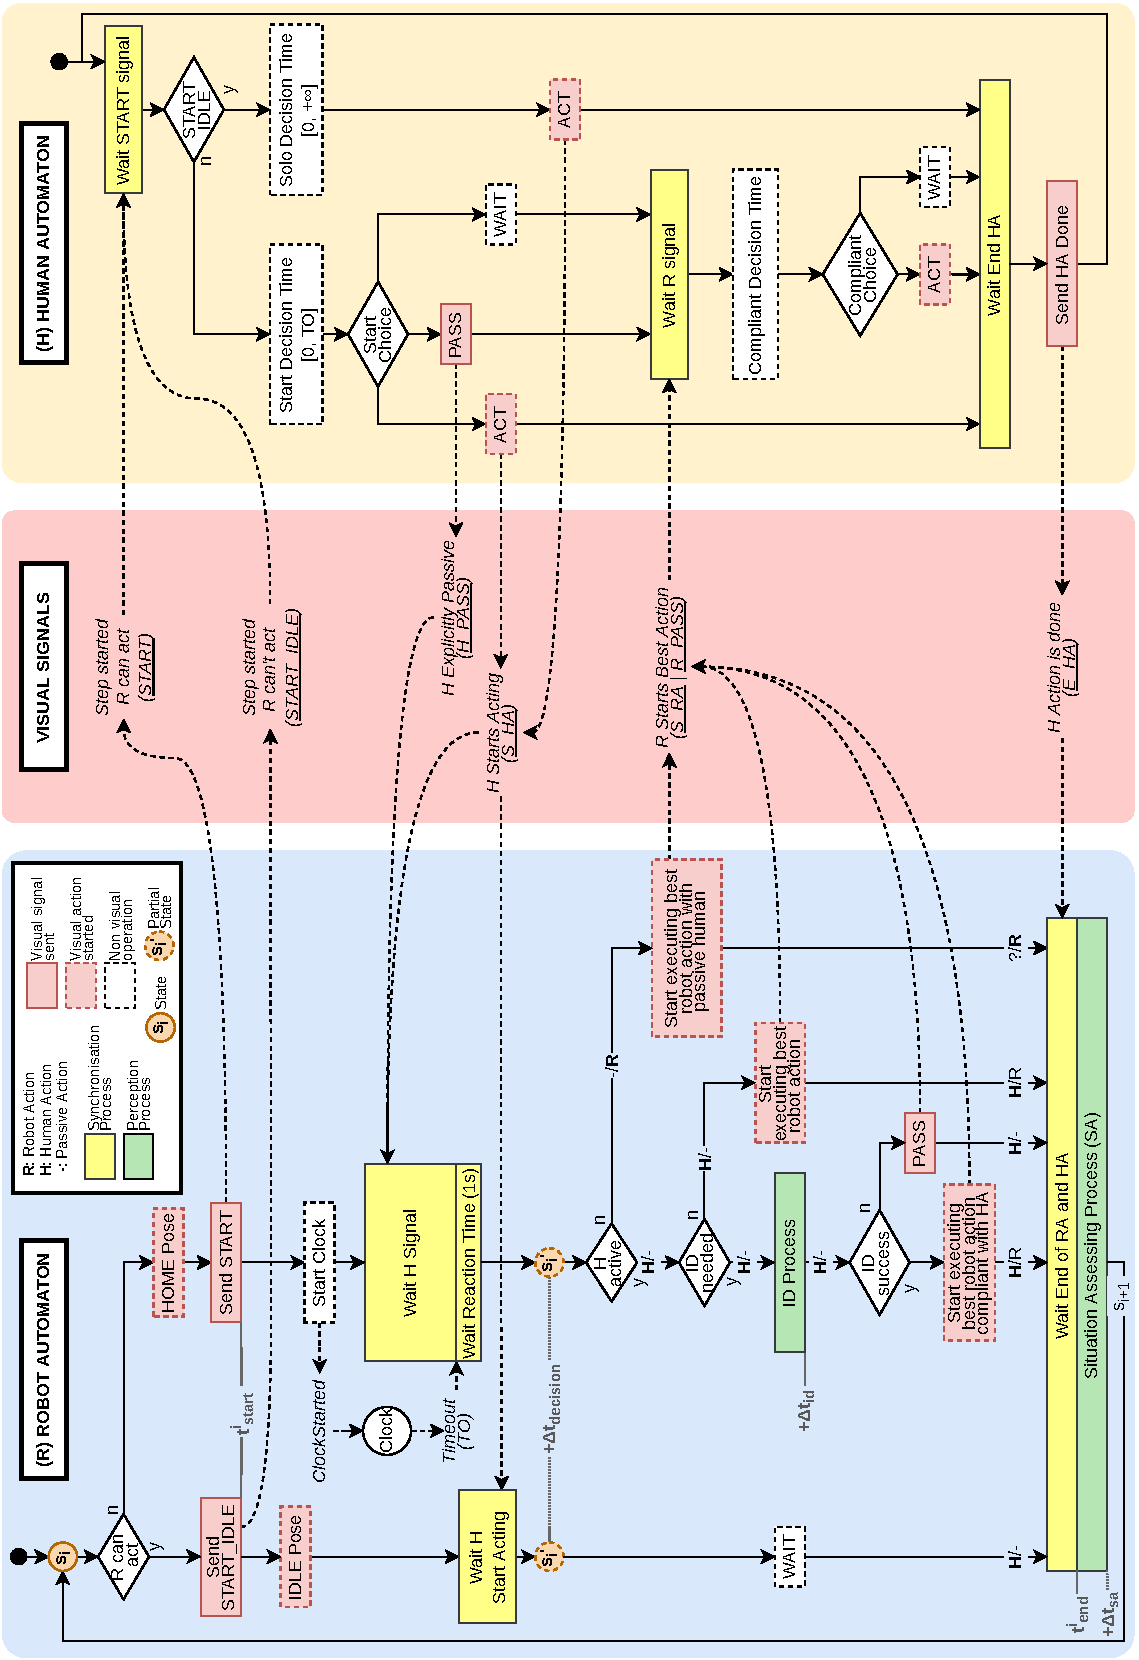
\includegraphics[width=0.99\linewidth]{Chapter5/complete_automaton_rotated.pdf}
    \caption{Complete Model of Execution - Dual Automaton. This version details the robot automaton and the assumed human automaton as well as the visual signals exchanges between the agents to synchronize themselves.}
    \label{fig:complete_model_exec}
\end{figure}

More precisely, \textit{describe differences between simplified and complete model}
\begin{itemize}
    \item ON robot automaton:
    \item HOME/IDLE pose (new left branch)
    \item Clock for TimeOut
    \item Robot Reaction Time
    \item branches 4-5 are merged and actually corresponds to compliant choice in human automaton
    \item Send Robot signals 
    \item Human Automaton: decision time, choices, wait signals
    \item Human signals
\end{itemize}

In the execution controller, the robot automaton is refined and more detailed. 
First, we show the social cues sent by the robot, which are the following: \textit{START} corresponds to the visual and audible signal indicating to the human that the step begins; \textit{S\_RA} corresponds to the start of a robot action; \textit{R\_PASS} corresponds to the robot being explicitly passive. The other signals, including the human ones, will be described below.
Also, we modeled the case where the robot cannot act in the current step. This can be determined easily given the search graph and the current state $s_i$ and by checking if there is at least one non-passive robot action in the following arcs. This checking process is represented in the figure by the diamond shape with the label ``R can act'', and the respective positive and negative answers ``yes'' (y) and ``no'' (n). When the robot cannot act, it sends a specific signal to inform the human that the step has started and cannot act (START\_IDLE), then goes in the \textit{IDLE} pose. This is a visually passive posture where the robot looks at the human with its arm retracted, indicating that it cannot act. Only a human action can progress to the next state. Thus, the robot waits for this action to start and eventually finish. Then, the Situation Assessment process identifies the executed action, and thus, the new state $s_{i+1}$ to continue. Depending on the possible actions, the robot can stay in this \textit{IDLE} pose for several steps. Once the robot can act again, the ``yes'' branch of the automaton is followed, and the robot returns to the \textit{HOME} pose. In this posture, the robot's arm is deployed, showing that the robot is ready to grab objects on the table.

Additionally, the process of waiting for a human signal at the beginning of each step is more detailed. This process is interrupted by one of the three following signals: \textit{H\_PASS} is an explicit signal (hand gesture, verbal communication) sent by the human to share its desire to be passive; \textit{S\_HA} is the start of human actions, and is detected by tracking human's motion; \textit{TO} is the internal timeout signal sent by a clock $4s$ after the start of the waiting process. 
However, the perception layer on a real robot would induce a delay for this synchronization process. 
An additional waiting time of $1s$ is added to compensate the robot's reaction time, allowing the human to send signals just before the timeout. Without it, the human could start moving just before the timeout, but the robot would interpret this information too late and consider them as passive.
Note that the robot only waits for a human signal if the human can act in the current step. This check is done similarly to is first diamond process. However, it is not shown in the figure for legibility reasons. Hence, it means that in situations where only the robot can act, it will not wait and will directly start acting.

% Remember that this process only identifies an explicit signal like a predefined hand gesture or the start of a human motion. In the case of human motion, we do not yet identify which action the human is starting. This is achieved by the dedicated Identification (ID) process, which is longer and here about $0.6s$. Thus, we believe that the chosen duration of $0.3s$ is relevant for detecting the initial human signals. 

The last visual difference with the abstracted model on the robot's side is the case where the human decides to be passive. In this branch, the human decision is pictured as a question mark. This is because we first identified the human as passive, and thus, the robot performs the best corresponding action provided by the policy. However, while the robot is acting, the human is free to start performing any action that does not conflict with the already started robot's action. These possible decisions are modeled in the human automaton described after but are identified by the robot only during the Situation Assessment process. 

On the other hand, a human automaton now explicitly models how humans should behave to coordinate with robots and collaborate successfully. This automaton starts by always waiting for the beginning of the current step, indicated by the robot with the signals \textit{START} or \textit{START\_IDLE}. The simplest but less common case is when the robot cannot act during the step (after receiving \textit{START\_IDLE}). This case is depicted in the rightmost branch. Since the robot cannot act, only the human can make progress in the task by acting. Thus, the human is free to take as much time as desired, represented by the decision time in the range $[0; +\infty]$. After the start of the human action, both human and robot automatons wait for the end of the human action, and then they proceed.
Let us discuss now the most common case where the robot can act. This time, the human must decide before the defined robot timeout (TO), otherwise they will be considered passive. The human can decide either to start acting (ACT), if possible in the current step, to indicate their passivity (PASS), or do nothing corresponding to being passive without informing the robot (WAIT). If the human decides to be passive (PASS or WAIT cases), they can either remain passive until the next step or decide to perform an action not conflicting with the robot one. This is represented with the last human diamond shape ``Compliant choice'' which is made after a duration referred to as ``compliant decision time''.


\section{Simulation controllers}

To control the simulated agents and the simulation, 4 distinct controllers have been developed and handle dedicated jobs. 

\subsection{Robot arm motion controller}

First, there is one controller to move the robot arm. This controller is called with either a 3D position to reach (pose target) or a predefined configuration (named target). In both cases, when called, this controller uses the MoveIt framework. MoveIt creates links between several libraries in order to have access to a unified interface for Motion Planning algorithms, Inverse Kinematics, Control, or Collision Checking. This way, our controller can ``simply'' request MoveIt to find a trajectory to a given position and then make the robot follow this trajectory while taking into account the geometry of the robot arm.

In fact, this controller is slightly more sophisticated. Indeed, in our collaborative context, we prefer the robot to be reactive rather than to have optimal motions. This is why, through the MoveIt interface, we use two different motion planners. The first one is $RRT^*$ which is an optimal planner that stops only when the optimal motion plan has been found. This is desirable to have the robot exhibit consistent and efficient motions. However, this process sometimes takes too much time (4-5s), which breaks the rhythm of the interaction. As a consequence, a short timeout (0.6s) has been set for this optimal motion planner. If the optimal plan isn't found within the defined timeout, we use the second motion planner. 
The second planner is $SBL$ which isn't an optimal planner. That is, the planner stops when a solution is found, but there is no guarantee of optionality. The major pro of this planner is its speed.
Overall, for every robot arm motion, we first try to find an optimal motion within a short amount of time. If the optimal motion isn't found, we quickly find a suboptimal solution to prevent the robot from being passive for too long.

Additionally, to reduce motion planning time, a few simplifications have been done. 
First, collisions are only considered with the table and the robot's body. Hence, the robot arm sometimes go through the other cubes.
Also, the pick and place orientation are ignored, for instance, when picking a cube the robot gripper just reaches the cube's center from any angle and then the cube is attached to the gripper. When placing a cube, the robot moves the cube to the target position and when dropping it, the cube is detached and both its orientation and position are overwritten to match the actual target location. This way, the robot always performs perfect place action, improving both the reactivity of the robot and its robustness, but the robot's motions are less realistic.

\subsection{Robot head motions}

To exhibit a more intuitive and collaborative behavior, the robot head is controlled to look at various elements during the interaction. 
Indeed, when waiting for the human the robot looks at the camera, and as soon as the human hand moves to either perform an action or indicate its passivity, the robot starts following the hand to show it is observing the human motions to understand their intentions.
Then, the robot looks at a cube to indicate its intention to pick it since this is faster than the arm motion. 
Also, the robot looks at the target position when placing a cube to indicate its intention to place the cube there.

To perform those head motions a dedicated controller has been developed based on an existing controller provided in the Tiago robot modules. The existing controller could only change the robot's gaze through a visual and clickable window allowing an operator to manually click on the scene to change the robot's gaze. This controller has been modified to allow additional features such as directly requesting to look at 3D point or an object. But also, we can now ask to follow an object. That's how we are able to exhibit the head behavior described just above.  

\subsection{Human hand motions}

Moving the human hand requires a dedicated controller but is much simpler than the robot arm motion one. Here, the hand must either move to a position or perform a PASS signal. The PASS signal is a hand gesture indicating to the robot that the human desires to be passive for the current step. This motion is performed by simply rotating the hand back and forth at a constant speed. The PASS motion has a duration of 0.7s. 
On the other hand, to move the hand to a target position we do not use a real motion planner. We simply compute a straight line between the current hand pose and the target pose, and update the hand position at $50Hz$ to move at a constant speed set to $0.25 m/s$. The planning time is thus negligible compared to the robot motion planning times.

\subsection{Simulation controller}

\subsubsection{Action decomposition}

Last but not least, I developed a fourth controller whose main job is to translate the actions from the plan produced by our task planner to low-level motions that can be executed by the controllers listed above. Hence, some parts of this controller are domain-specific, but a major part is generic for manipulation tasks. This controller received high-level agent actions to execute such as ``Robot pick(b1)'' for the robot picking the cube b1. The first step is to decompose this action into low-level generic actions which are themselves made of low-level motions. This controller also keeps track of a few low-level facts to check low-level preconditions, such as, what are each agent holding or which object is still on the table. Hence, when an agent tries to pick a cube while already holding a cube the controller throws an error.

Let's first comment the low-level generic actions available. This controller is given a list of the object names (cubes) and the names of some predefined locations in the scene (placing locations in the stack). Note also that many of the following actions can be performed either by the human or the robot, this is defined by a parameter given when calling the action. The following low-level actions are available:

\begin{itemize}
    \itemsep0em
    \item \textbf{move\_pose\_target:}          moves either the hand/robot arm to a given position.
    \item \textbf{move\_location\_target:}      moves either the hand/robot arm to the position of a given location.
    \item \textbf{move\_obj\_target:}           moves the hand/robot arm to the position of a given object.
    \item \textbf{move\_home:}                  puts the agent in its ``home'' (default) configuration. 
    \item \textbf{move\_named\_target:}         moves the robot arm to the given configuration.
    \item \textbf{grab\_obj:}                   attaches the given object to the hand/robot gripper. 
    \item \textbf{drop\_obj:}                   detaches the given object to the hand/robot gripper.
    \item \textbf{set\_obj\_rpy:}               sets the orientation of a given object.
    \item \textbf{set\_obj\_pose:}              sets the position of a given object.
    \item \textbf{delta\_move\_obj:}            sets the position of a given relative to its current position.
    \item \textbf{human\_hand\_gesture:}        makes a hand gesture to indicate passivity.
    \item \textbf{robot\_head\_look\_pose:}     makes the robot look at a given position.
    \item \textbf{robot\_head\_look\_human:}    makes the robot look at the human (camera).
    \item \textbf{robot\_head\_follow\_obj:}    makes the robot follow a given object.
    \item \textbf{robot\_head\_follow\_hand:}   makes the robot follow the human hand.
\end{itemize}

Then the high-level actions, from the plan produced, are the following with their respective simplified low-level decomposition:

\begin{itemize}
    \item \textbf{PickCube:}            Starts by retrieving the cube's current position by sending a request to the Gazebo simulator. If it is the robot, call robot\_head\_look\_obj to look at the cube. Then, call move\_pose\_target with the retrieved cube position. Once over, grab the cube with grab\_obj. After, move\_home is called to retract the robot arm or bring the hand to its initial position. Finally, if it is the robot, it looks to the human with robot\_head\_look\_human.
    
    \item \textbf{PlaceCube:}           Starts by retrieving the position of the target location to stack the cube. If it is the robot, call robot\_head\_look\_pose with this position. Then, we move either the arm or the hand to that position with move\_pose\_target before dropping the cube in the stack with drop\_obj and adjusting its position. After, we go back to the home configuration with move\_home. And for the robot, we look at the human with robot\_head\_look\_human. 
    
    \item \textbf{BePassive:}           The human waves their hand to explicitly be passive, thus, human\_hand\_gesture is called. The robot doesn't move and only display some texts saying the robot wants to be passive. The text prompt mechanism will be described later.
    
    \item \textbf{DropCubeTable:}       When an agent cannot stack a cube they are holding, they can place it back on the table. First, the drop position is defined. It corresponds to the initial position of the cube being held, except for the green one which is initially on top of another cube and has a dedicated drop position. The robot looks at the drop position with robot\_head\_follow\_pose. The hand or the robot arm is moved to the position with move\_pose\_target. The cube is dropped with drop\_obj and its position is adjusted. Then, the agent is put in its home configuration with move\_home, and the robot looks at the human with robot\_head\_look\_human.  
\end{itemize}

\subsubsection{Manage steps}

One last thing, the simulator controller is in charge of indicating when a step is over. Basically, since we do not consider steps where both agents are passive, a step begins when an agent starts an action. And it is over when both agent actions are done. These rules cover many situations such as if the human initially wants to be passive and wave their hand, as a result, the robot starts performing an action which starts the step. Currently, the step would be over as soon as the robot action is over since the human is passive. However, if the human decides anyway to start performing an action concurrently then the step will be over when both the robot and human actions are over. This may imply that if the human starts acting right before the end of the robot action then the robot will just wait for the end of the human action, and thus, the end of the step before the next step begins.  

\subsubsection{Send visual signals}

The model of execution synchronizes the agents based on explicit visual signals such as the start of a step, the start of an action, the end of an action, or hand gesture (PASS). Those signals are modeled explicitly inside the system and managed by the simulator controller.

Indeed, when starting an action, the associated visual signal is sent only when the agent starts to move. Hence, we track the arm and hand motions to know when the action is visible to the other agent. Then, when an action is over, the associated visual signal is sent directly. It is worth mentioning that humans will naturally have a reaction time when seeing the robot's visual signals (start/end of action, step start). However, the robot natively does not have any reaction time to such symbolic visual signals. Thus, to simulate the delay introduced by an actual perception module (here perfectly simulated), the human visual signals are delayed to the robot by a reaction time set to 0.3 seconds. This is still quite fast, but at least the robot does not interpret human motions instantly.   




\section{Human Machine Interface (HMI)}

\textbf{TODO: to develop}

text prompt, clickable zones, signals

Human operator or participant can interact with the simulation by performing any feasible action during the process. The model of execution is still followed, thus, every step starts by the robot sound and a dedicated process receives internally the list of the feasible human actions for the current step. This list is sent by the robot execution scheme which is reading the solution graph. Yet, the feasible actions aren't shown nor known by the participants.
Each possible human action is associated to a zone (rectangle) on the screen. When the human mouse click in a zone associated to a currently feasible action, then the process request the simulation controller to perform the corresponding human action.  delayed visual signal for robot.

\section{Logs and timeline}

There is also a dedicated process to record the different events and signals during one execution. All other components can send events to log to this process to save them for later post-processing. A log event is defined with a name and a time stamp. Additionally, visual signals are also captured by this logging process and saved them both as a signal and creates an associated event. Logged events mostly help to trace the internal states and processes ran by the robot during the execution. The human ones mostly only serve to identify when the human is acting or not since we don't have access to the internal reasoning process of the human participant. 

\subsection{Activities extraction}

All logs are saved after each execution and can be loaded later for post-processing. The post-processing involve three steps. First, the agent activities are extracted from the event list. The human and the robot have different possible activities, but again, since we don't have access to the internal human reasoning there are more robot activities than human ones. The extracted activities are shown in the following table~\ref{tab:agent_activities}. The activities orders try to match what can happen during the execution but not all activities are present in every step. Indeed, on the robot side, the ID process isn't always necessary and thus not always executed, and the robot either perform an action or is passive for diverse reasons. But the robot always end up waiting for the end of the step, perform the SA process and get ready for the next step. On the human side, if the human performs an action or make a hand gesture, there will be a decision time than respectively the human action or the explicit passive activity. If the human remains passive without signaling the robot then the only activity is passive without signaling. Only if the human is active, the waiting next step to start activity is added, otherwise being passive for a step is implicitly equivalent to waiting for the next step.  

\begin{table}[]
    \begin{tabular}{|l|l|}
    \hline
    \multicolumn{1}{|c|}{\textbf{Robot Activities}}                                           & \multicolumn{1}{c|}{\textbf{Human Activities}}                                                       \\ \hline
    Waiting for human decision                                                                & Decision Time                                                                                        \\ \hline
    Identification Process (ID process)                                                       & \multirow{3}{*}{Human Action}                                                                        \\ \cline{1-1}
    Planning arm motion                                                                       &                                                                                                      \\ \cline{1-1}
    Robot Action                                                                              &                                                                                                      \\ \hline
    \begin{tabular}[c]{@{}l@{}}Waiting for human action when\\ itself cannot act\end{tabular} & \begin{tabular}[c]{@{}l@{}}Being passive with signaling \\ (after PASS hand gesture)\end{tabular}    \\ \hline
    Being passive                                                                             & \begin{tabular}[c]{@{}l@{}}Being passive without signaling\\ (after TimeOut is reached)\end{tabular} \\ \hline
    Waiting for the end of the step                                                           & \multirow{3}{*}{Waiting for the next step to start}                                                  \\ \cline{1-1}
    Situation Assessment Process (SA process)                                                 &                                                                                                      \\ \cline{1-1}
    Getting ready for the next step (GRNS)                                                    &                                                                                                      \\ \hline
    \end{tabular}
    \caption{Agent activities extracted from logs. The activities orders and relative positions try to match the execution but not all activities are present in every step.  }
    \label{tab:agent_activities}
    \end{table}

\subsection{Metrics computation}

When loading the execution logs we extract a set of metrics from the events and extracted activities. Currently, 27 metrics are extracted, but the following table \ref{tab:metrics} only shows 11 because several sub-metrics are hidden. Indeed, for four of the listed metrics, we compute the sum, average, standard deviation, min, and max values of the corresponding metric.

% {\small
% \begin{enumerate}
%     \itemsep0em
%     \item \textbf{Task completion time:}                 Time for the stack to be completed.
%     \item \textbf{Number of steps:}                      Number of steps executed.
%     \item \textbf{Number of human optimal actions:}      Number of human action being optimal regarding a given objective.
%     \item \textbf{Ratio of human optimal actions:}       Number of human optimal actions divided by the number of steps.
%     \item \textbf{Decision time:}                        Time for the human to make a visible decision in a step. Five different metrics are extracted regarding all steps of the scenario: total/sum, average, standard deviation, min and max.
%     \item \textbf{Waiting Next Step:}                    Time during which the human waits for the next step to start. Again, are extracted over all the steps: total, average, standard deviation, min and max values.
%     \item \textbf{Number of human action:}               Number of human actions executed in the scenario.
%     \item \textbf{Human action duration:}                Over all steps are extracted the total, average, standard deviation, min and max duration of the human actions.
%     \item \textbf{Number of robot action:}               Number of robot actions executed in the scenario.
%     \item \textbf{Robot action duration:}                Over all steps are extracted the total, average, standard deviation, min and max duration of the robot actions.
%     \item \textbf{Time human free:}                      Time after which the human is free, i.e., isn't mandatory for the task to be completed.
% \end{enumerate}
% }

\begin{table}[]
    \begin{tabular}{|c|l|}
    \hline
    \textbf{Metric}                                                           & \multicolumn{1}{c|}{\textbf{Description}}                                                                                   \\ \hline
    Task Completion Time                                                      & Time for the task to eh completed.                                                                                          \\ \hline
    Number of steps                                                           & Number of steps executed.                                                                                                   \\ \hline
    \begin{tabular}[c]{@{}c@{}}Number of optimal\\ human actions\end{tabular} & \begin{tabular}[c]{@{}l@{}}Number of human action being optimal regarding a \\ given objective.\end{tabular}                \\ \hline
    \begin{tabular}[c]{@{}c@{}}Ratio of optimal\\ human actions\end{tabular}  & \begin{tabular}[c]{@{}l@{}}Number of optimal human action divided by the \\ number of steps.\end{tabular}                   \\ \hline
    Human decision time*                                                      & \begin{tabular}[c]{@{}l@{}}Duration for the human to make a visible decision \\ in a step.\end{tabular}                     \\ \hline
    Waiting next step*                                                        & \begin{tabular}[c]{@{}l@{}}Duration during which the human waits for the next \\ step to start.\end{tabular}                \\ \hline
    \begin{tabular}[c]{@{}c@{}}Number of \\ human action\end{tabular}         & \begin{tabular}[c]{@{}l@{}}Number of non-passive human actions executed in \\ the scenario.\end{tabular}                    \\ \hline
    \begin{tabular}[c]{@{}c@{}}Human action \\ duration*\end{tabular}         & Duration of the human actions.                                                                                              \\ \hline
    \begin{tabular}[c]{@{}c@{}}Number of \\ robot action\end{tabular}         & \begin{tabular}[c]{@{}l@{}}Number of non-passive robot actions executed in \\ the scenario.\end{tabular}                    \\ \hline
    \begin{tabular}[c]{@{}c@{}}Robot action \\ duration*\end{tabular}         & Duration of the robot actions.                                                                                              \\ \hline
    Time human free                                                           & \begin{tabular}[c]{@{}l@{}}Time after which the human is free, i.e., as soon as \\ the robot can finish alone.\end{tabular} \\ \hline
    \end{tabular}
    \caption{Metrics extracted from the execution logs for each scenario. Marked items with a star (*) correspond to five sub-metrics computed over all steps: sum, average, standard deviation, min, and max values.}
    \label{tab:metrics}
    \end{table}

\subsection{Execution example with timeline}

A complete scenario is presented and commented on in this section. Using the previously extracted agent activities, we can draw a visual timeline depicting the different steps, the extracted activities, and the visual signals exchanged between the agents. Figure \ref{fig:timeline_example} depicts the complete commented timeline, including agents' activities, exchanged signals, and snapshots from the simulator. The table \ref{tab:signals} describes the different signals exchanged during the execution and shown on the timeline. 

\begin{table}[h]
    \begin{tabular}{|c|l|}
    \hline
    \textbf{Signal name} & \multicolumn{1}{c|}{\textbf{Description}}                                                                                        \\ \hline
    START                & \begin{tabular}[c]{@{}l@{}}Visual and audible signal from the robot indicating that the\\ current step has started.\end{tabular} \\ \hline
    START\_IDLE          & \begin{tabular}[c]{@{}l@{}}Visual and audible signal indicating the start of a step where\\ the robot cannot act.\end{tabular}   \\ \hline
    S\_RA / E\_RA        & \begin{tabular}[c]{@{}l@{}}Signals sent respectively from the start (S) and the end (E) of \\ a robot action (RA).\end{tabular}  \\ \hline
    S\_HA / E\_HA        & \begin{tabular}[c]{@{}l@{}}Signals sent respectively from the start (S) and the end (E) of\\ a human action (HA).\end{tabular}   \\ \hline
    H\_PASS              & \begin{tabular}[c]{@{}l@{}}Explicit hand gesture from the human informing their desire\\ the be passive.\end{tabular}            \\ \hline
    TO                   & \begin{tabular}[c]{@{}l@{}}The TimeOut is an internal robot signal indicating that the \\ absence of human signal.\end{tabular}  \\ \hline
    \end{tabular}
    \caption{Signals exchanged between the agents during the execution and used for synchronization and coordination.}
    \label{tab:signals}
    \end{table}

\begin{figure}
    \centering
    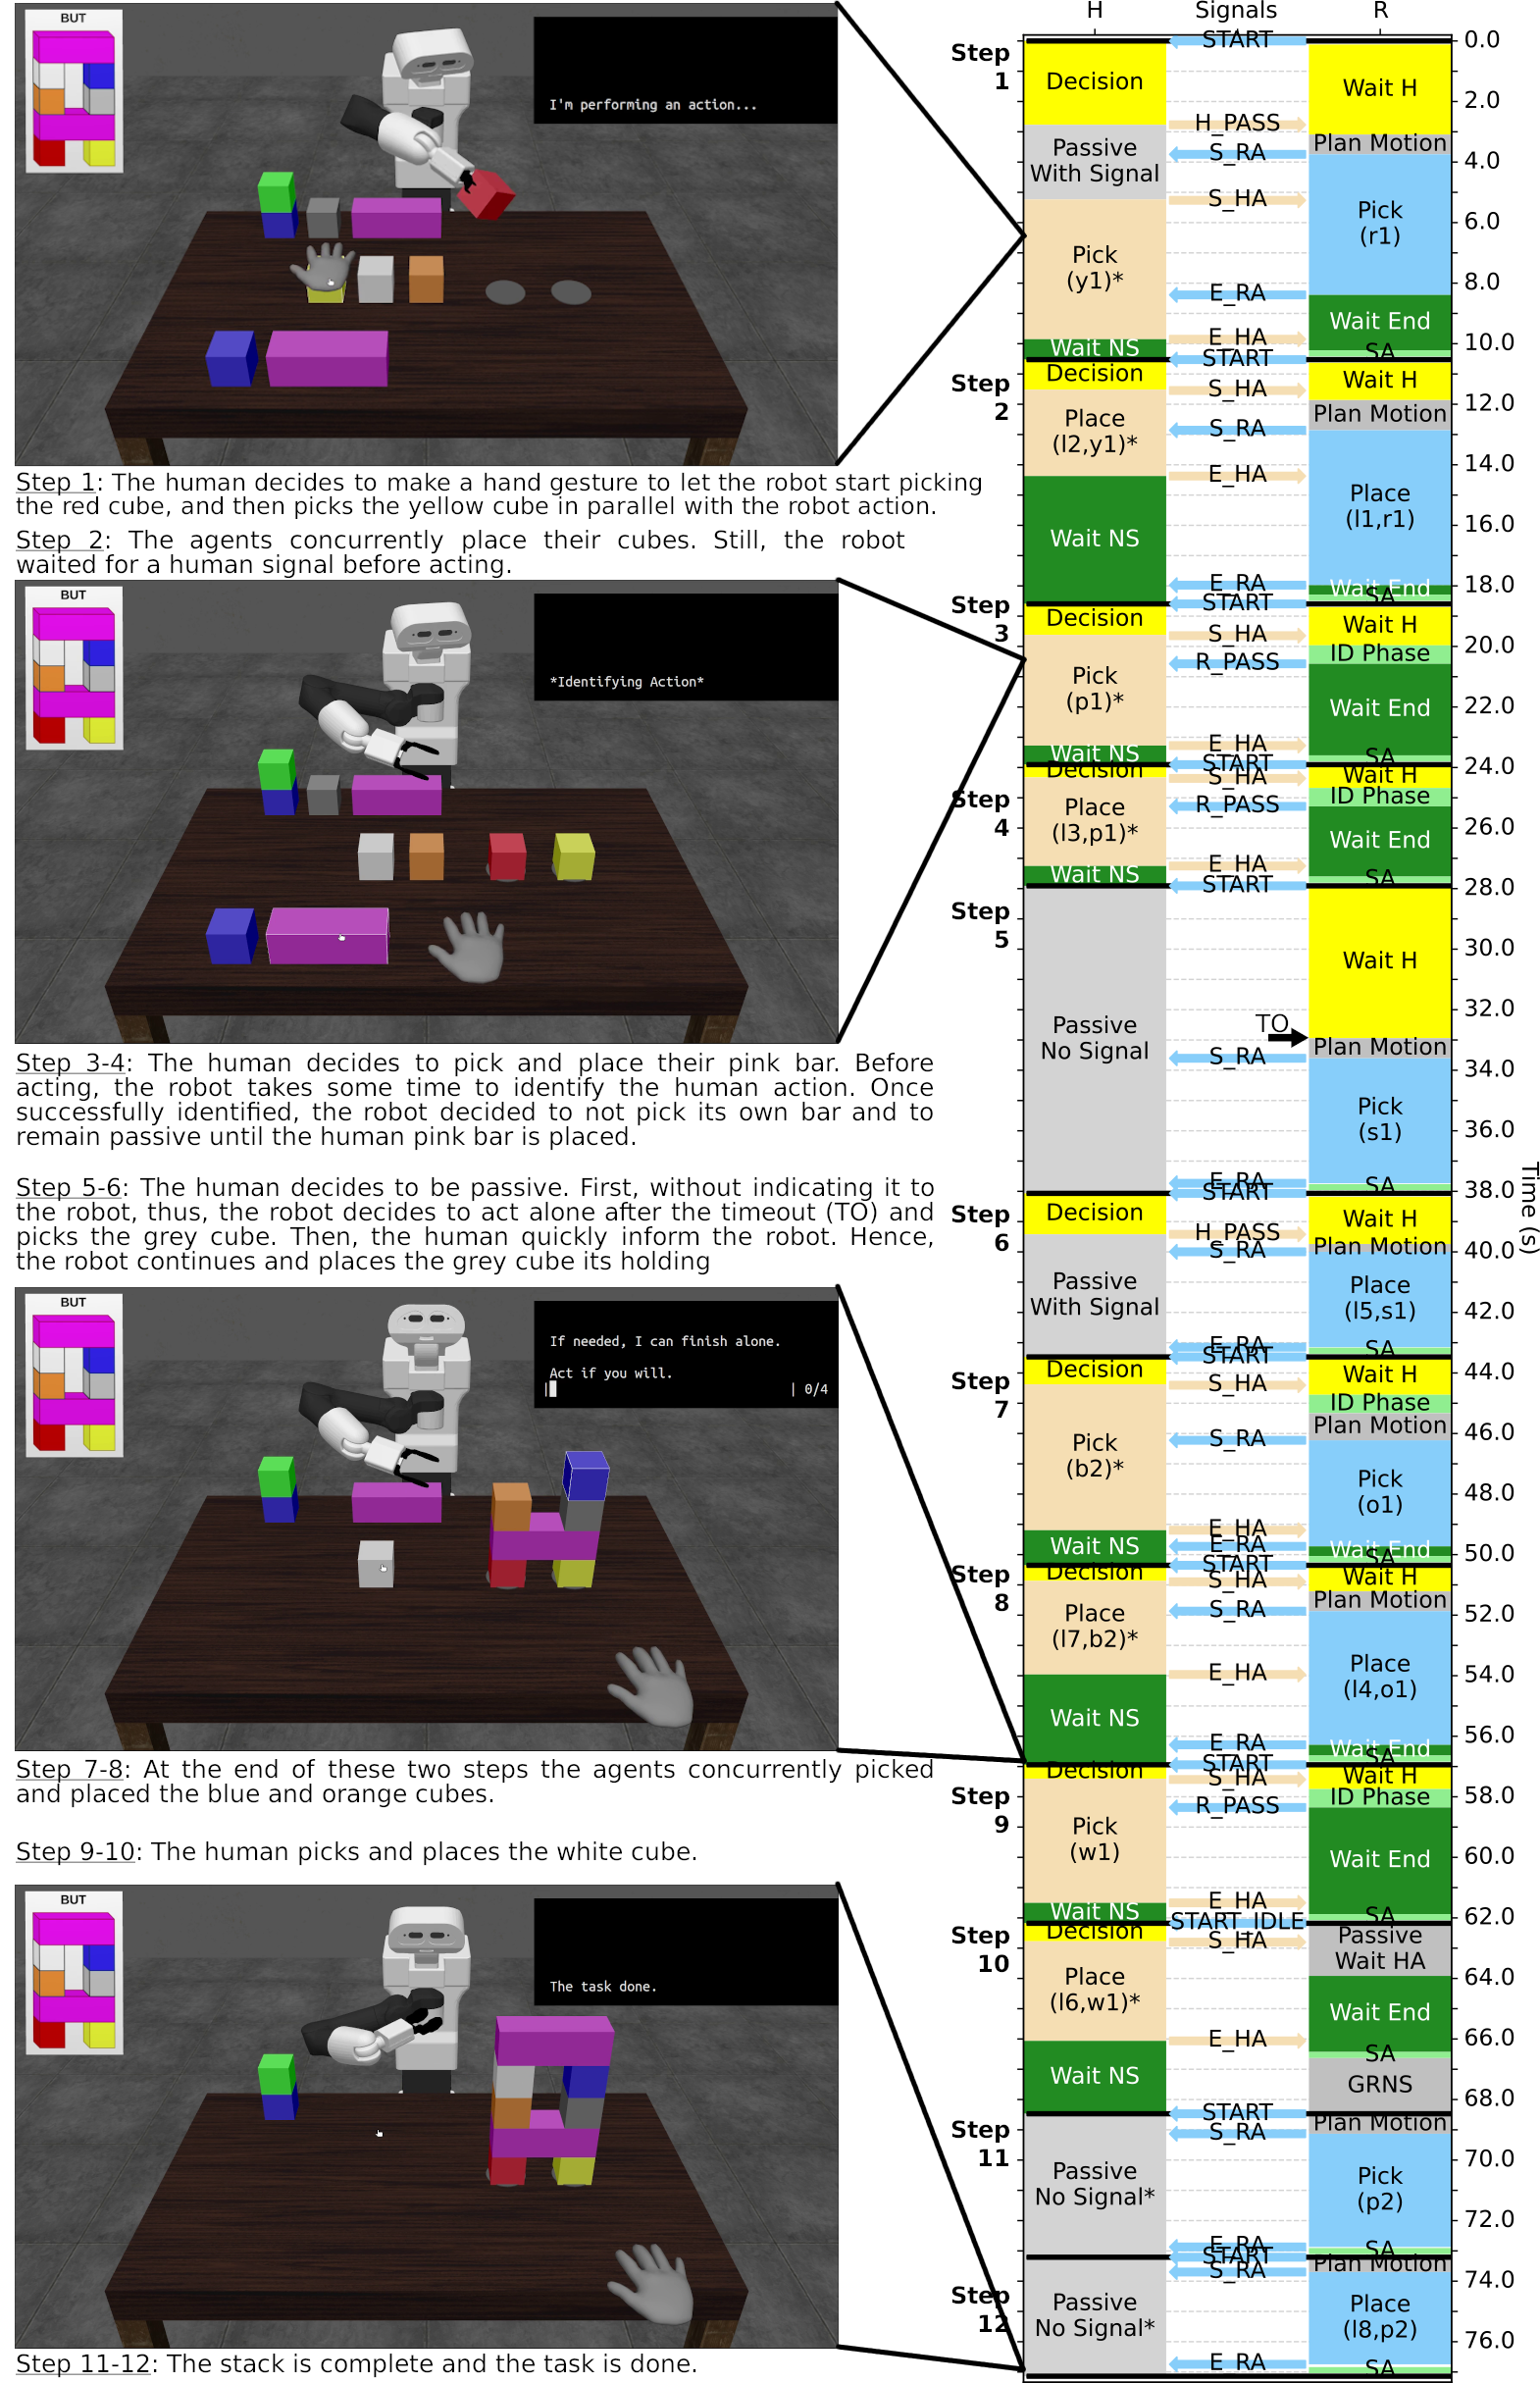
\includegraphics[height=0.97\textheight, keepaspectratio]{Chapter5/last_timeline.png}
    \caption{Complete execution timeline commented.}
    \label{fig:timeline_example}
\end{figure}

In this execution example, according to the extracted metrics, the task has been completed in $77.14s$ in $12$ steps. The average human decision time is $1.00s \pm 0.69s$ with $max=2.77s$ and $min=0.42s$. The human waited on average for the start of the next step during $1.68s \pm 1.28s$. There were $8$ human actions with an average duration of $3.67s \pm 0.72s$. According to the objective/preferences to finish the task as fast as possible, the human acted $9$ times optimally out of $12$ steps (optimal ratio$=75\%$). Indeed, the human agent purposely decided to be passive during steps 5 and 6, but they could have picked the orange cube in parallel to complete the stack faster. In this example, the task description forbids agents from picking cubes in advance. They must be able to immediately place a cube in the stack to pick it. This rule is detailed and justified later in the next chapter \ref{sec:study_protocol}. Hence, in step 9, the human picked the white cube, but the robot could not pick the bar until the white cube was placed. Thus, the human could have let the robot place the white cube to reduce their effort without slowing the task.
There were $8$ robot actions with an average duration of $3.97s \pm 0.69s$. Overall, the robot took $5.25s$ to plan its arm motions. 


